%% LyX 2.0.3 created this file.  For more info, see http://www.lyx.org/.
%% Do not edit unless you really know what you are doing.
\documentclass[10pt]{beamer}\usepackage[]{graphicx}\usepackage[]{color}
%% maxwidth is the original width if it is less than linewidth
%% otherwise use linewidth (to make sure the graphics do not exceed the margin)
\makeatletter
\def\maxwidth{ %
  \ifdim\Gin@nat@width>\linewidth
    \linewidth
  \else
    \Gin@nat@width
  \fi
}
\makeatother

\definecolor{fgcolor}{rgb}{0.345, 0.345, 0.345}
\newcommand{\hlnum}[1]{\textcolor[rgb]{0.686,0.059,0.569}{#1}}%
\newcommand{\hlstr}[1]{\textcolor[rgb]{0.192,0.494,0.8}{#1}}%
\newcommand{\hlcom}[1]{\textcolor[rgb]{0.678,0.584,0.686}{\textit{#1}}}%
\newcommand{\hlopt}[1]{\textcolor[rgb]{0,0,0}{#1}}%
\newcommand{\hlstd}[1]{\textcolor[rgb]{0.345,0.345,0.345}{#1}}%
\newcommand{\hlkwa}[1]{\textcolor[rgb]{0.161,0.373,0.58}{\textbf{#1}}}%
\newcommand{\hlkwb}[1]{\textcolor[rgb]{0.69,0.353,0.396}{#1}}%
\newcommand{\hlkwc}[1]{\textcolor[rgb]{0.333,0.667,0.333}{#1}}%
\newcommand{\hlkwd}[1]{\textcolor[rgb]{0.737,0.353,0.396}{\textbf{#1}}}%

\usepackage{framed}
\makeatletter
\newenvironment{kframe}{%
 \def\at@end@of@kframe{}%
 \ifinner\ifhmode%
  \def\at@end@of@kframe{\end{minipage}}%
  \begin{minipage}{\columnwidth}%
 \fi\fi%
 \def\FrameCommand##1{\hskip\@totalleftmargin \hskip-\fboxsep
 \colorbox{shadecolor}{##1}\hskip-\fboxsep
     % There is no \\@totalrightmargin, so:
     \hskip-\linewidth \hskip-\@totalleftmargin \hskip\columnwidth}%
 \MakeFramed {\advance\hsize-\width
   \@totalleftmargin\z@ \linewidth\hsize
   \@setminipage}}%
 {\par\unskip\endMakeFramed%
 \at@end@of@kframe}
\makeatother

\definecolor{shadecolor}{rgb}{.97, .97, .97}
\definecolor{messagecolor}{rgb}{0, 0, 0}
\definecolor{warningcolor}{rgb}{1, 0, 1}
\definecolor{errorcolor}{rgb}{1, 0, 0}
\newenvironment{knitrout}{}{} % an empty environment to be redefined in TeX

\usepackage{alltt}
\usepackage[T1]{fontenc}
\setcounter{secnumdepth}{3}
\setcounter{tocdepth}{3}
\usepackage{color}
\usepackage{colortbl}
\usepackage{dcolumn}
\usepackage{amsmath}
\usepackage{tikz}
\usepackage{floatflt}
\usepackage{multicol}
\usepackage{multirow}
\usepackage{listings}
\usepackage{tabularx}
\usepackage{amssymb}% http://ctan.org/pkg/amssymb
\usepackage{pifont}% http://ctan.org/pkg/pifont
\usepackage{bbm}
\usepackage{siunitx}
\usepackage{url}
\usepackage{verbatim}
\usepackage{enumerate}
\usepackage{algorithmic}
\usepackage[flushleft]{threeparttable}
\usepackage{algorithm}
\usepackage{hyperref}
\hypersetup{
    colorlinks,%
    citecolor=blue,%
    filecolor=blue,%
    linkcolor=blue,%
    urlcolor=blue}
\ifx\hypersetup\undefined
  \AtBeginDocument{%
    \hypersetup{unicode=true,pdfusetitle,
 bookmarks=true,bookmarksnumbered=false,bookmarksopen=false,
 breaklinks=false,pdfborder={0 0 0},backref=false,colorlinks=false}
  }
\else
  \hypersetup{unicode=true,pdfusetitle,
 bookmarks=true,bookmarksnumbered=false,bookmarksopen=false,
 breaklinks=false,pdfborder={0 0 0},backref=false,colorlinks=false}
\fi

\makeatletter

%%%%%%%%%%%%%%%%%%%%%%%%%%%%%% LyX specific LaTeX commands.
\providecommand{\LyX}{\texorpdfstring%
  {L\kern-.1667em\lower.25em\hbox{Y}\kern-.125emX\@}
  {LyX}}


%%%%%%%%%%%%%%%%%%%%%%%%%%%%%% Textclass specific LaTeX commands.
 % this default might be overridden by plain title style
 \newcommand\makebeamertitle{\frame{\maketitle}}%
 \AtBeginDocument{
   \let\origtableofcontents=\tableofcontents
   \def\tableofcontents{\@ifnextchar[{\origtableofcontents}{\gobbletableofcontents}}
   \def\gobbletableofcontents#1{\origtableofcontents}
 }
 \def\lyxframeend{} % In case there is a superfluous frame end
 \long\def\lyxframe#1{\@lyxframe#1\@lyxframestop}%
 \def\@lyxframe{\@ifnextchar<{\@@lyxframe}{\@@lyxframe<*>}}%
 \def\@@lyxframe<#1>{\@ifnextchar[{\@@@lyxframe<#1>}{\@@@lyxframe<#1>[]}}
 \def\@@@lyxframe<#1>[{\@ifnextchar<{\@@@@@lyxframe<#1>[}{\@@@@lyxframe<#1>[<*>][}}
 \def\@@@@@lyxframe<#1>[#2]{\@ifnextchar[{\@@@@lyxframe<#1>[#2]}{\@@@@lyxframe<#1>[#2][]}}
 \long\def\@@@@lyxframe<#1>[#2][#3]#4\@lyxframestop#5\lyxframeend{%
   \frame<#1>[#2][#3]{\frametitle{#4}#5}}

\renewcommand{\footnotesize}{\fontsize{6pt}{6pt}\selectfont}

%%%%%%%%%%%%%%%%%%%%%%%%%%%%%% User specified LaTeX commands.
%\usetheme{Warsaw}
\usetheme{Boadilla}
%\setbeamertemplate{navigation symbols}{}
%gets rid of bottom navigation bars
%\setbeamertemplate{footline}[page number]{}
%\setcounter{page}{44}
%\setbeamertemplate{footline}{}


\makeatother
\IfFileExists{upquote.sty}{\usepackage{upquote}}{}

\begin{document}


\title[Bayesian Hierarchical Time Series]{Bayesian Hierarchical Time Series}
\author[Leo Guelman]{Leo Guelman}
\institute[]{}
\date[December 2020]{Tech Talk\\  DNA \\ RBC Royal Bank}

\makebeamertitle

\lyxframeend{}


%%%%Slide

\begin{frame}
[fragile]\frametitle{A Metaphor...}

\begin{itemize} 

\item Read Richard McElreth 

\item Example decision tree, or flowchart, for selecting an appropri- ate statistical procedure. Beginning at the top, the user answers a series of questions about measurement and intent, arriving eventually at the name of a procedure. Many such decision trees are possible.

\item Something similar to ML

\item Probably I should put each use case a label : Prediction / Counterfactuals / Inference / Instrumental Variables (well this os not the objective but the method is to solve a problem) 

\item What is the goal of this presentation?

\begin{itemize} 

\item Often cases, thinking about the data generating process (the underlying mechanism that generated the observed data)?

\item When is this important? Think about noisy settings (with low signal to noise ratio), limited data, or when we want to predict under intervention (as opposed to under observation) 

\item Contrast to using domain knowledge vs end-to-end ML o  make predictions? 

\end{itemize} 

\end{itemize} 
 
  
\end{frame}

%%%%Slide

\begin{frame}
[fragile]\frametitle{A Model for Golf Putting}


\begin{columns}[T] % align columns
\begin{column}{.48\textwidth}

\begin{itemize}

\vskip10pt

\item Aggregate data\footnotemark from professional golfers, showing the proportion of successful putts as a function of distance.

\item Error bars associated to each point $j$ are classical standards deviations $\sqrt{\hat{p_j}(1-\hat{p_j})/n_j}$.

\end{itemize}

\end{column}%
\hfill%
\begin{column}{.48\textwidth}

\begin{figure}
   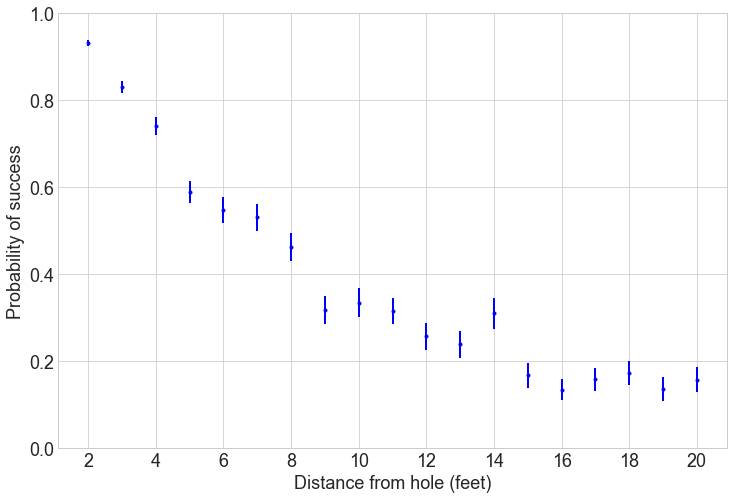
\includegraphics[width= 0.9\linewidth]{figures/golf1.png}
\end{figure}

\end{column}%
\end{columns}

\footnotetext[1]{Source: Don Berry’s 1996 textbook (Statistics, A Bayesian Perspective)}

\end{frame}


%%%%Slide

\begin{frame}
[fragile]\frametitle{A Model for Golf Putting -- Logistic Regression}


\begin{columns}[T] % align columns
\begin{column}{.48\textwidth}

\underline{The Model}

\begin{align*}
y_j & \sim \text{Binomial}(n_j, p_j) \\
\text{logit}(p_j) & = a + bx_j;~\text{for}~j =  \{1, \ldots, J\} \\
a & \sim \text{Normal}(0,1) \\
b & \sim \text{Normal}(0,1) \\
\end{align*}

\pause

\end{column}%
\hfill%
\begin{column}{.48\textwidth}

\begin{figure}
   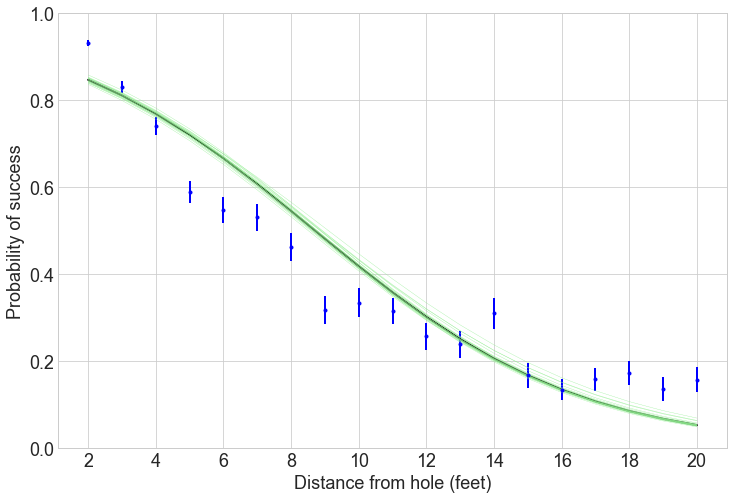
\includegraphics[width= 0.9\linewidth]{figures/golf2a.png}
\end{figure}

\end{column}%
\end{columns}

\vskip20pt

\begin{figure}
   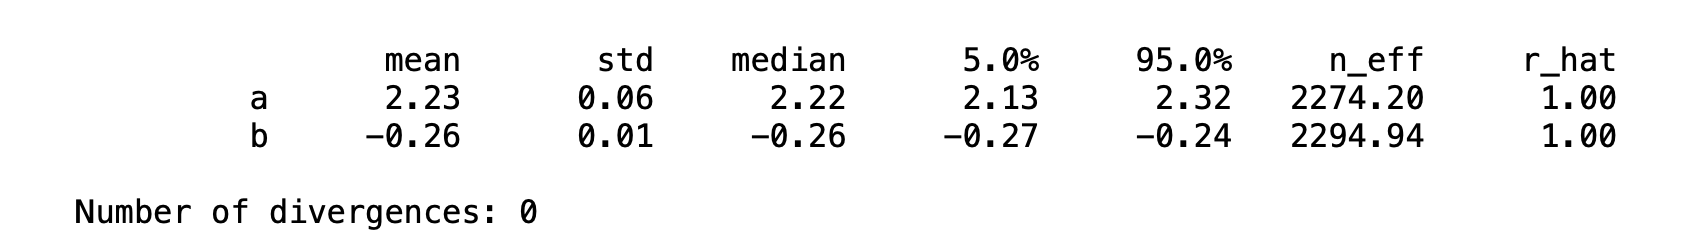
\includegraphics[width= 0.9\linewidth]{figures/golf2b.png}
\end{figure}
  
\end{frame}


%%%%Slide

\begin{frame}
[fragile]\frametitle{A Model for Golf Putting -- Principled Approach}

\begin{itemize}

\item The dotted line represents the angle within which the ball of radius $r$ must be hit so that it falls within the hole of radius $R$. 

\begin{figure}
   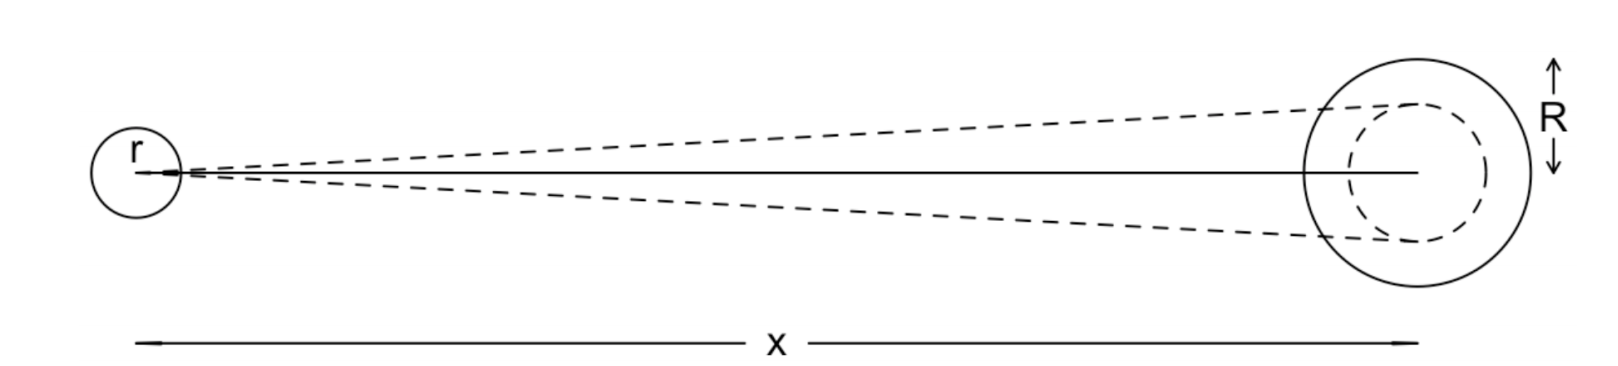
\includegraphics[width= 0.9\linewidth]{figures/golf3.png}
\end{figure}

\vskip5pt

\item The threshold angle is given by  $\text{sin}^{-1} ((R - r)/ x)$.

\vskip5pt

\item Next, we need to model the human error:

\begin{equation*}
 \text{Angle} \sim \text{Normal}(0,\sigma)
 \end{equation*}

\vskip5pt

\item The probability the ball goes in the hole $\Rightarrow$ Probability that the angle is less than the threshold


\begin{equation*}
\text{Pr} \big( \lvert{\text{angle}}  \lvert  \le \text{sin}^{-1} \big((R - r)/ x \big) \big)= 2 \Phi  \Bigg(\frac{\text{sin}^{-1} \big((R - r)/ x\big)}{\sigma} \Bigg) - 1 
\end{equation*}

\end{itemize}


\end{frame}



%%%%Slide

\begin{frame}
[fragile]\frametitle{A Model for Golf Putting -- Principled Model (cont'd)}


\begin{columns}[T] % align columns
\begin{column}{.48\textwidth}

\underline{The Model}

\begin{align*}
y_j & \sim \text{Binomial}(n_j, p_j) \\
p_j & = 2\Phi \Bigg( \frac{ \text{sin}^{-1} \big((R - r)/ x_j \big) }{\sigma}  \Bigg) - 1 
\end{align*}

where $r$=1.68; $R$=4.25 inches.

\pause

\end{column}%
\hfill%
\begin{column}{.48\textwidth}

\begin{figure}
   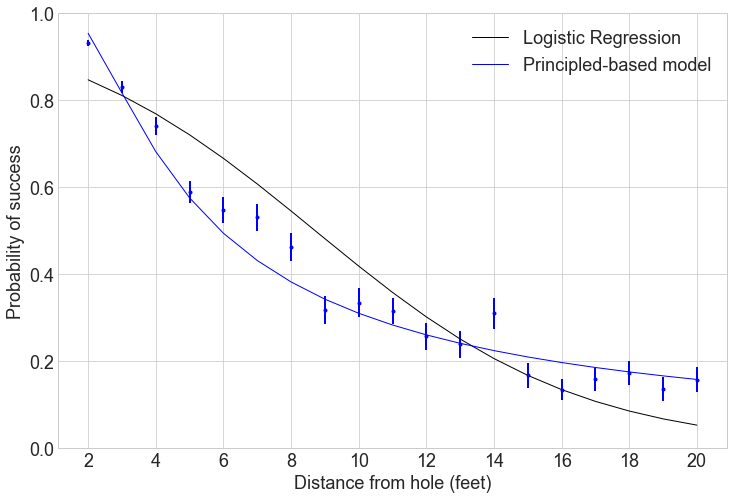
\includegraphics[width= 0.9\linewidth]{figures/golf4a.png}
\end{figure}

\end{column}%
\end{columns}


\begin{figure}
   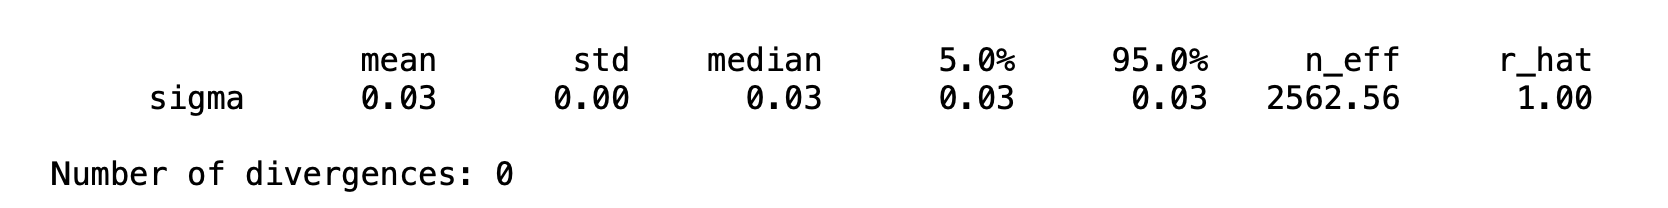
\includegraphics[width= 0.9\linewidth]{figures/golf4b.png}
\end{figure}


 \end{frame}
 
 
 %%%%Slide

\begin{frame}
[fragile]\frametitle{A Client Attrition Model}

\begin{itemize}

\item \textbf{Consider the following problem}: we are tasked to build a client attrition model for RBC Visa Avion Cards, and we find the following ``insight'':

\vskip10pt

\begin{figure}
   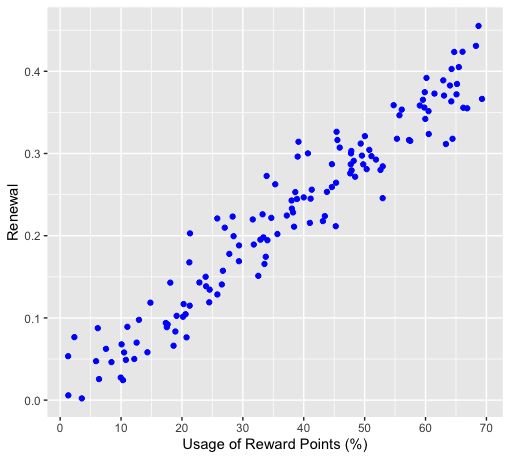
\includegraphics[width= 0.4\linewidth]{figures/renewal1.png}
\end{figure}

\vskip10pt

\item \textbf{What is our best prediction of renewal} if: 

\begin{enumerate}

\item we were to observe a client using 90\% of her reward points?

\item  create an incentive program to promote usage, and get this client to use 90\% of her reward points?

\end{enumerate}


\end{itemize}

 \end{frame}
 
 
 
 %%%%Slide

\begin{frame}
[fragile]\frametitle{A Client Attrition Model (cont'd)}


\begin{itemize}

\item \textbf{Case 1} is a well-studied problem in ML: we just need to fit a model and use it to make a prediction under the new $X$ (renewal points). 

\item  \textbf{Case 2} requires us to think about the data generating process, and in particular, the optimal prediction should depend on the underlying causal structure.

\pause

\begin{figure}
   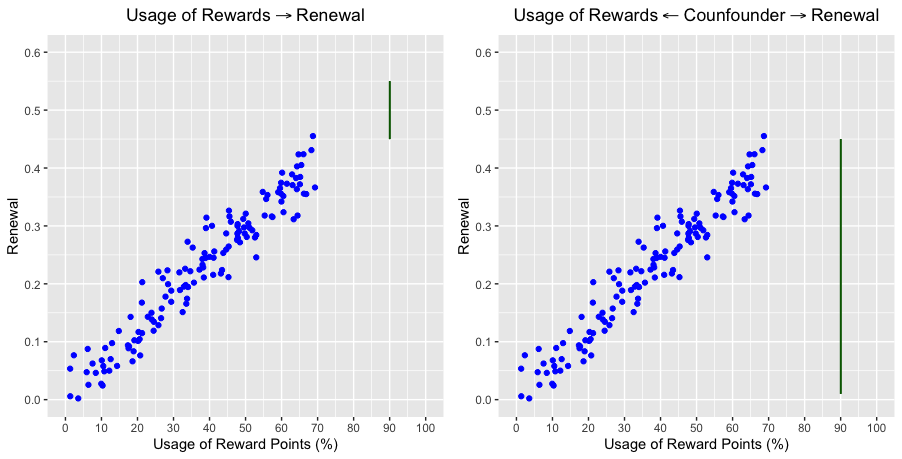
\includegraphics[width= 0.8\linewidth]{figures/renewal2.png}
\end{figure}


\item If we do not accept any form of causal notion, we cannot distinguish between these two cases and our best prediction must be: ``I do not know.''!

\end{itemize}



 \end{frame}
 
\end{document}

